\documentclass[10pt,a4paper]{article}
\usepackage[margin=21mm,headheight=14pt]{geometry}
\usepackage{fontspec}
\setmainfont{Times New Roman}
\setsansfont{Avenir Next}
\setmonofont{Menlo}[Scale=0.83]
\newfontfamily\devanagarifont{Devanagari Sangam MN}
\newfontfamily\bengalifont{Kohinoor Bangla}
\newfontfamily\kannadafont{Kannada Sangam MN}
\newfontfamily\gujaratifont{Gujarati Sangam MN}
\newfontfamily\tamilfont{Tamil Sangam MN}
\newfontfamily\telugufont{Telugu Sangam MN}
\usepackage{graphicx}
\usepackage{booktabs,longtable,array,tabularx}
\usepackage{microtype}
\usepackage{xcolor}
\usepackage{caption}
\usepackage{fancyhdr}
\usepackage{hyperref}
\hypersetup{colorlinks=true,linkcolor=blue!40!black,urlcolor=blue!40!black,
  pdftitle={Terminus Lean 150M: 10B-token dense FP8 run report},
  pdfauthor={Terminus research}}
\definecolor{TerminusBlue}{HTML}{17324D}
\definecolor{TerminusGray}{HTML}{627080}
\captionsetup{font=small,labelfont=bf}
\setlength{\parskip}{0.35em}
\setlength{\parindent}{0pt}
\setlength{\emergencystretch}{3em}
\setlength{\tabcolsep}{4pt}
\renewcommand{\arraystretch}{1.12}
\renewcommand{\familydefault}{\rmdefault}
\newcommand{\tightlist}{\setlength{\itemsep}{0pt}\setlength{\parskip}{0pt}}
\pagestyle{fancy}
\fancyhf{}
\fancyhead[L]{\sffamily\footnotesize Terminus Lean 150M / Dense FP8}
\fancyhead[R]{\sffamily\footnotesize Final-run analysis}
\fancyfoot[C]{\sffamily\footnotesize\thepage}
\renewcommand{\headrulewidth}{0.3pt}
\setcounter{secnumdepth}{2}
\setcounter{tocdepth}{2}
\begin{document}
\begin{titlepage}
\vspace*{19mm}
{\sffamily\color{TerminusBlue}\LARGE Terminus Lean 150M\\[4mm]
\Huge Dense FP8 Training Run\\[3mm]
\Large Final Checkpoint and Stability Report\par}
\vspace{14mm}
{\large 10-billion-token experiment · 2 October 2026\par}
\vspace{12mm}
\rule{\linewidth}{0.7pt}
\vspace{5mm}
\begin{tabularx}{\linewidth}{@{}lX@{}}
Model & 146,423,680 trainable parameters; 25 layers; width 640\\
Training & 9,999,998,976 tokens; 25,432 updates; one H100 NVL\\
Final held-out loss & 2.4194 mixture-weighted; 2.7597 English\\
Numerical integrity & 0 non-finite incidents; 254 clipped updates\\
Artifacts & 257 validation points; 2,546 stability probes; 23 prompt completions
\end{tabularx}
\vspace{5mm}
\rule{\linewidth}{0.7pt}
\vspace{12mm}
\textbf{Assessment.} The run completed and held-out loss improved in every
tracked source. The checkpoint remains weak on several simple factual, arithmetic,
and code-completion probes. The first attention RMSNorm gain shrank markedly and
final-layer residual scale grew, despite finite gradients and improving loss.
Those scale signals warrant a controlled continuation before QAT selection.
\par\vfill
{\small\color{TerminusGray}Run ID: \texttt{lean\_dense\_10b\_20261001}\\
Training code: \texttt{c95a951d5436489b8b0902e96b327adcaa11b524}\\
Final checkpoint SHA-256: \path{3d116e88048c93a0403ab2920b1680b066a9f29cbc07fa8ae1c2c67f2144684b}\\
Full run files: verified in Azure Blob; the H100 VM is deallocated.}
\end{titlepage}
\tableofcontents
\clearpage
\section{Verdict}\label{verdict}

The run converged numerically and its held-out token loss improved
across every tracked source. The final mixture-weighted validation loss
is \textbf{2.4194} and English is \textbf{2.7597}. Most of the late
improvement arrived during the 8B--10B learning-rate decay. That result
supports the value of finishing the schedule, but this one run does not
establish that the chosen learning rates, batch, or decay length are
optimal.

The final checkpoint is \textbf{not yet a reliable task-completion
model}. In a fixed 23-prompt greedy probe it answered some simple
prompts, including a Q\&A-form France-capital question and
\texttt{2\ +\ 2}, but failed \texttt{12\ +\ 19}, the freezing point of
water, several capital clozes, and sustained code completion. Many
outputs became repetitive. This is a 146M-parameter base language model
with no instruction tuning; held-out next-token loss is not a substitute
for task accuracy.

One numerical signal merits a controlled follow-up before treating this
checkpoint as an uncomplicated QAT starting point: the \textbf{first
attention RMSNorm gain collapsed from RMS 1.0 to 0.0165}, while the
sampled final-layer residual grew from RMS 0.61 near initialization to
34.37 at the end. Loss never diverged and the residual scale fell
substantially during decay, so this is not proof of a failed run. It is
an unusual learned scale regime, and the copied \texttt{norm\_lr=0.01}
is a plausible contributor that this run alone cannot identify causally.

\section{What ran and how loss was
measured}\label{what-ran-and-how-loss-was-measured}

The model has 146,423,680 trainable parameters, 25 layers, width 640, a
65,536-piece frozen tokenizer, four 512-token local-attention layers per
global-attention layer, dense FP8 projection arithmetic with FP32 master
weights, and Muon for projection matrices. It used BF16 residuals, main
block RMSNorms, no SubLN, and no Q/K normalization. The run used one
H100 NVL, microbatch 48, two gradient-accumulation steps, 4,096-token
sequences, and a nominal \textbf{393,216 training tokens per optimizer
update}. The last update was partial (122,880 tokens). The WSD schedule
used 1B-token warmup, 7B stable tokens, and 2B cosine decay to 10\% of
peak learning rate. The peak projection, embedding, and normalization
base learning rates were set to 0.01, with Muon matrix-specific scaling;
normalization vectors were in the auxiliary AdamW group with no weight
decay.

Each validation event scored \textbf{1,572,864 held-out tokens per
source} for English, code, math, and seven Indic languages. The overall
loss below is the source-loss mean weighted by the recorded training
mixture: 50\% English, 10\% code, 10\% math, and 30\% Indic (4.2--4.3\%
per Indic language). It is not the unweighted average of the ten
displayed losses. All losses are mean negative log-likelihood per
tokenizer token. A low code loss does not imply code-task competence;
domains have different predictability and the prompt test shows the
distinction.

\section{Loss trajectory}\label{loss-trajectory}

{
\begin{longtable}[]{@{}rrrrrrr@{}}
\toprule\noalign{}
Training tokens & Update & Weighted validation & English & Indic
weighted & Code & Math \\
\midrule\noalign{}
\endhead
\bottomrule\noalign{}
\endlastfoot
0.983B & 2,500 & 3.0214 & 3.3194 & 3.6726 & 0.9834 & 1.6162 \\
5.000B & 12,716 & 2.7788 & 3.0977 & 3.3335 & 0.8481 & 1.4508 \\
7.982B & 20,300 & 2.7566 & 3.0798 & 3.2978 & 0.8364 & 1.4372 \\
9.005B & 22,900 & 2.6190 & 2.9477 & 3.1157 & 0.7606 & 1.3442 \\
10.000B & 25,432 & \textbf{2.4194} & \textbf{2.7597} & \textbf{2.8525} &
\textbf{0.6389} & \textbf{1.1989} \\
\end{longtable}
}

The first validation, at 39.3M training tokens, was 5.8878 overall. The
first and last individual training-batch losses were 11.5818 and 2.4190;
individual batches are noisy and are not directly comparable to held-out
validation points.

The weighted loss fell 0.265 between the end of warmup and roughly 8B
tokens, then \textbf{0.337 in the 2B-token decay}. English fell 0.320
during decay. Every Indic stream improved by 0.417--0.461 over that
interval. The lowest recorded weighted validation was 2.41845 at update
25,400; the final value is only 0.00093 higher, well within the small
variation visible in adjacent checks. There is no sustained late
validation reversal.

\begin{figure}[htbp]
\centering
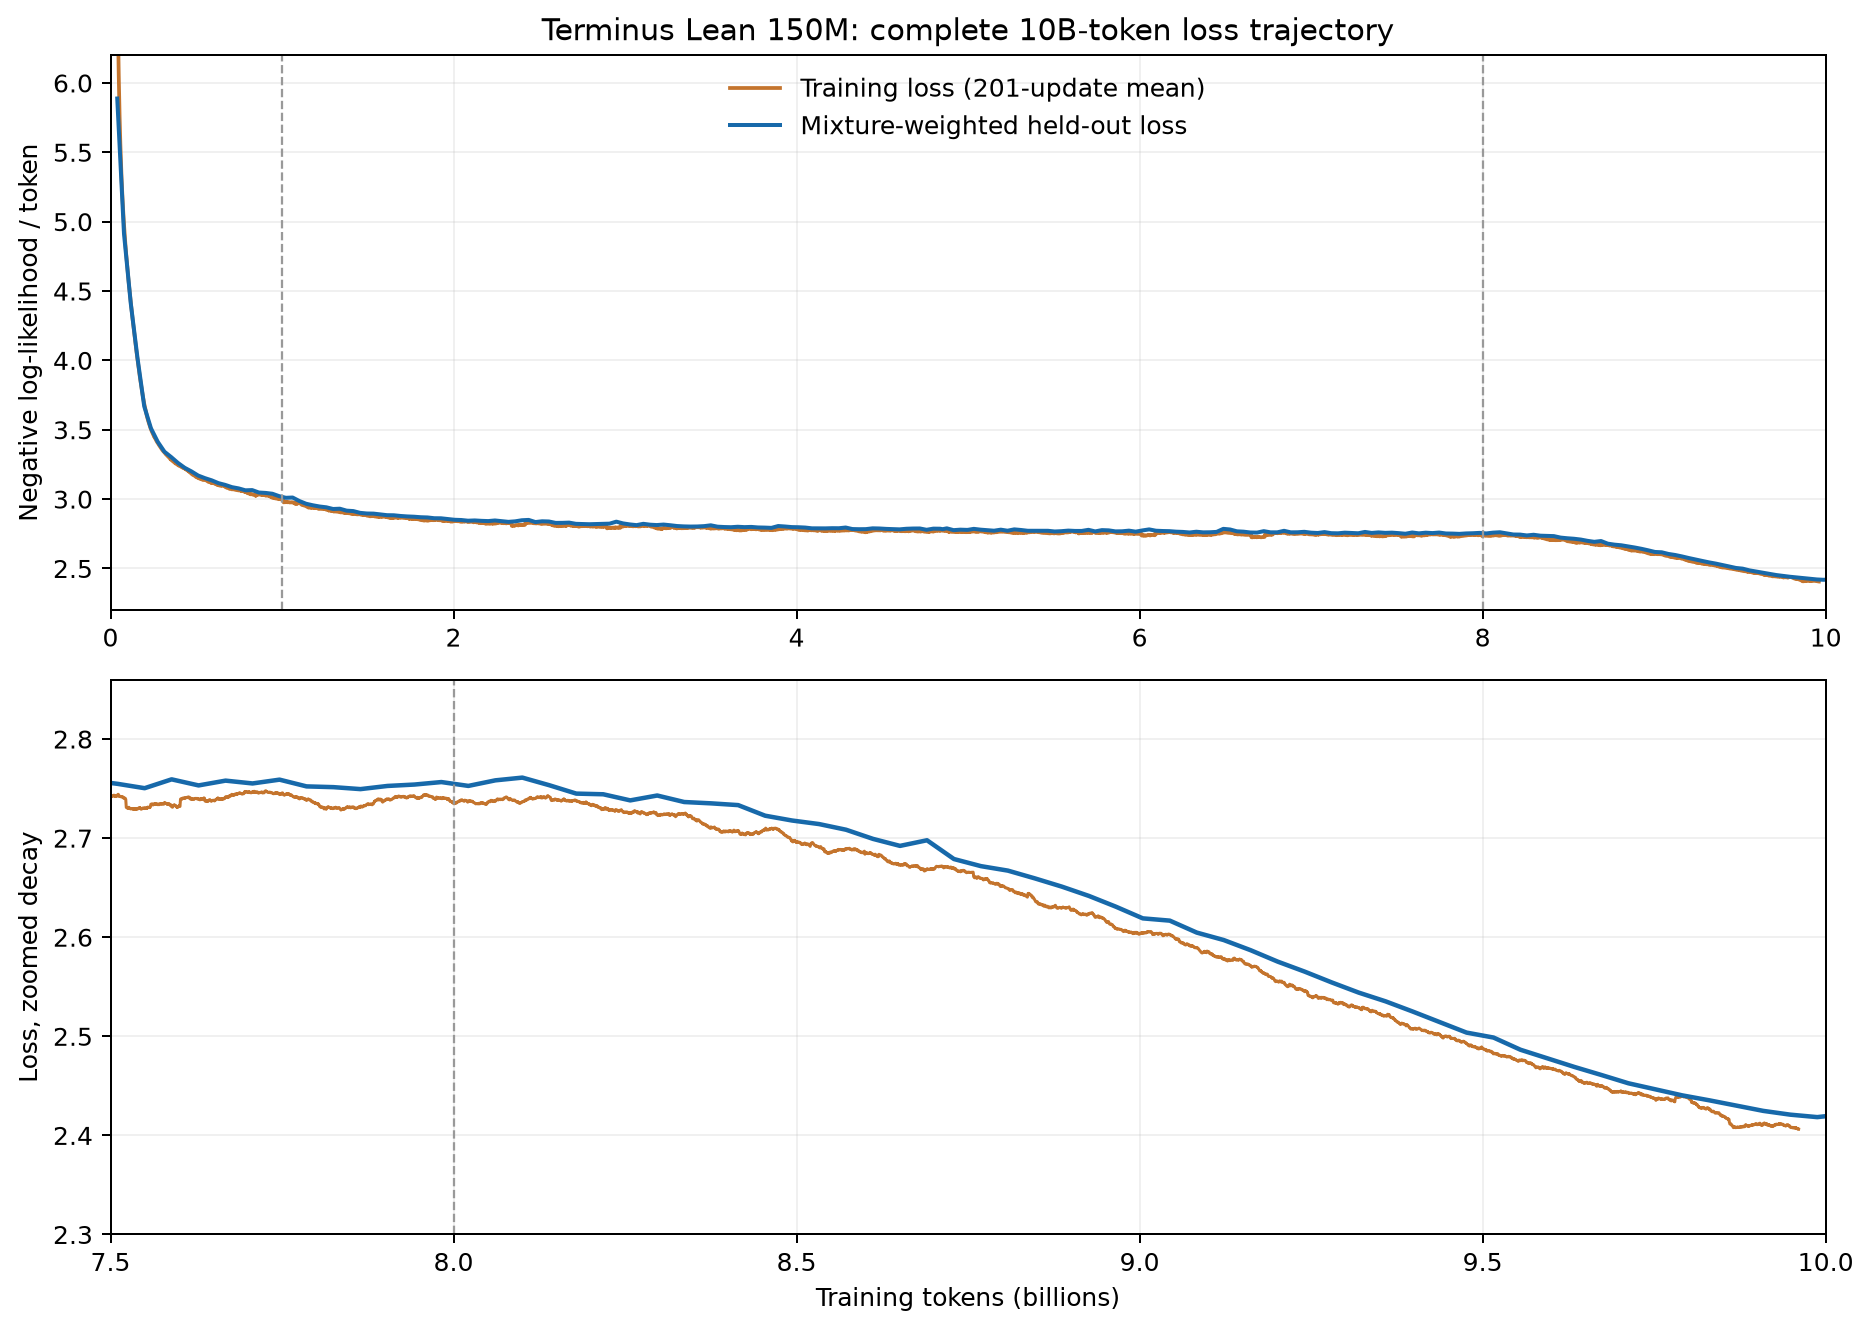
\includegraphics[width=0.96\linewidth]{figures/loss_overall.png}
\caption{Mixture-weighted held-out loss over all 10B training tokens, with a late-run zoom.}
\end{figure}

\begin{figure}[htbp]
\centering
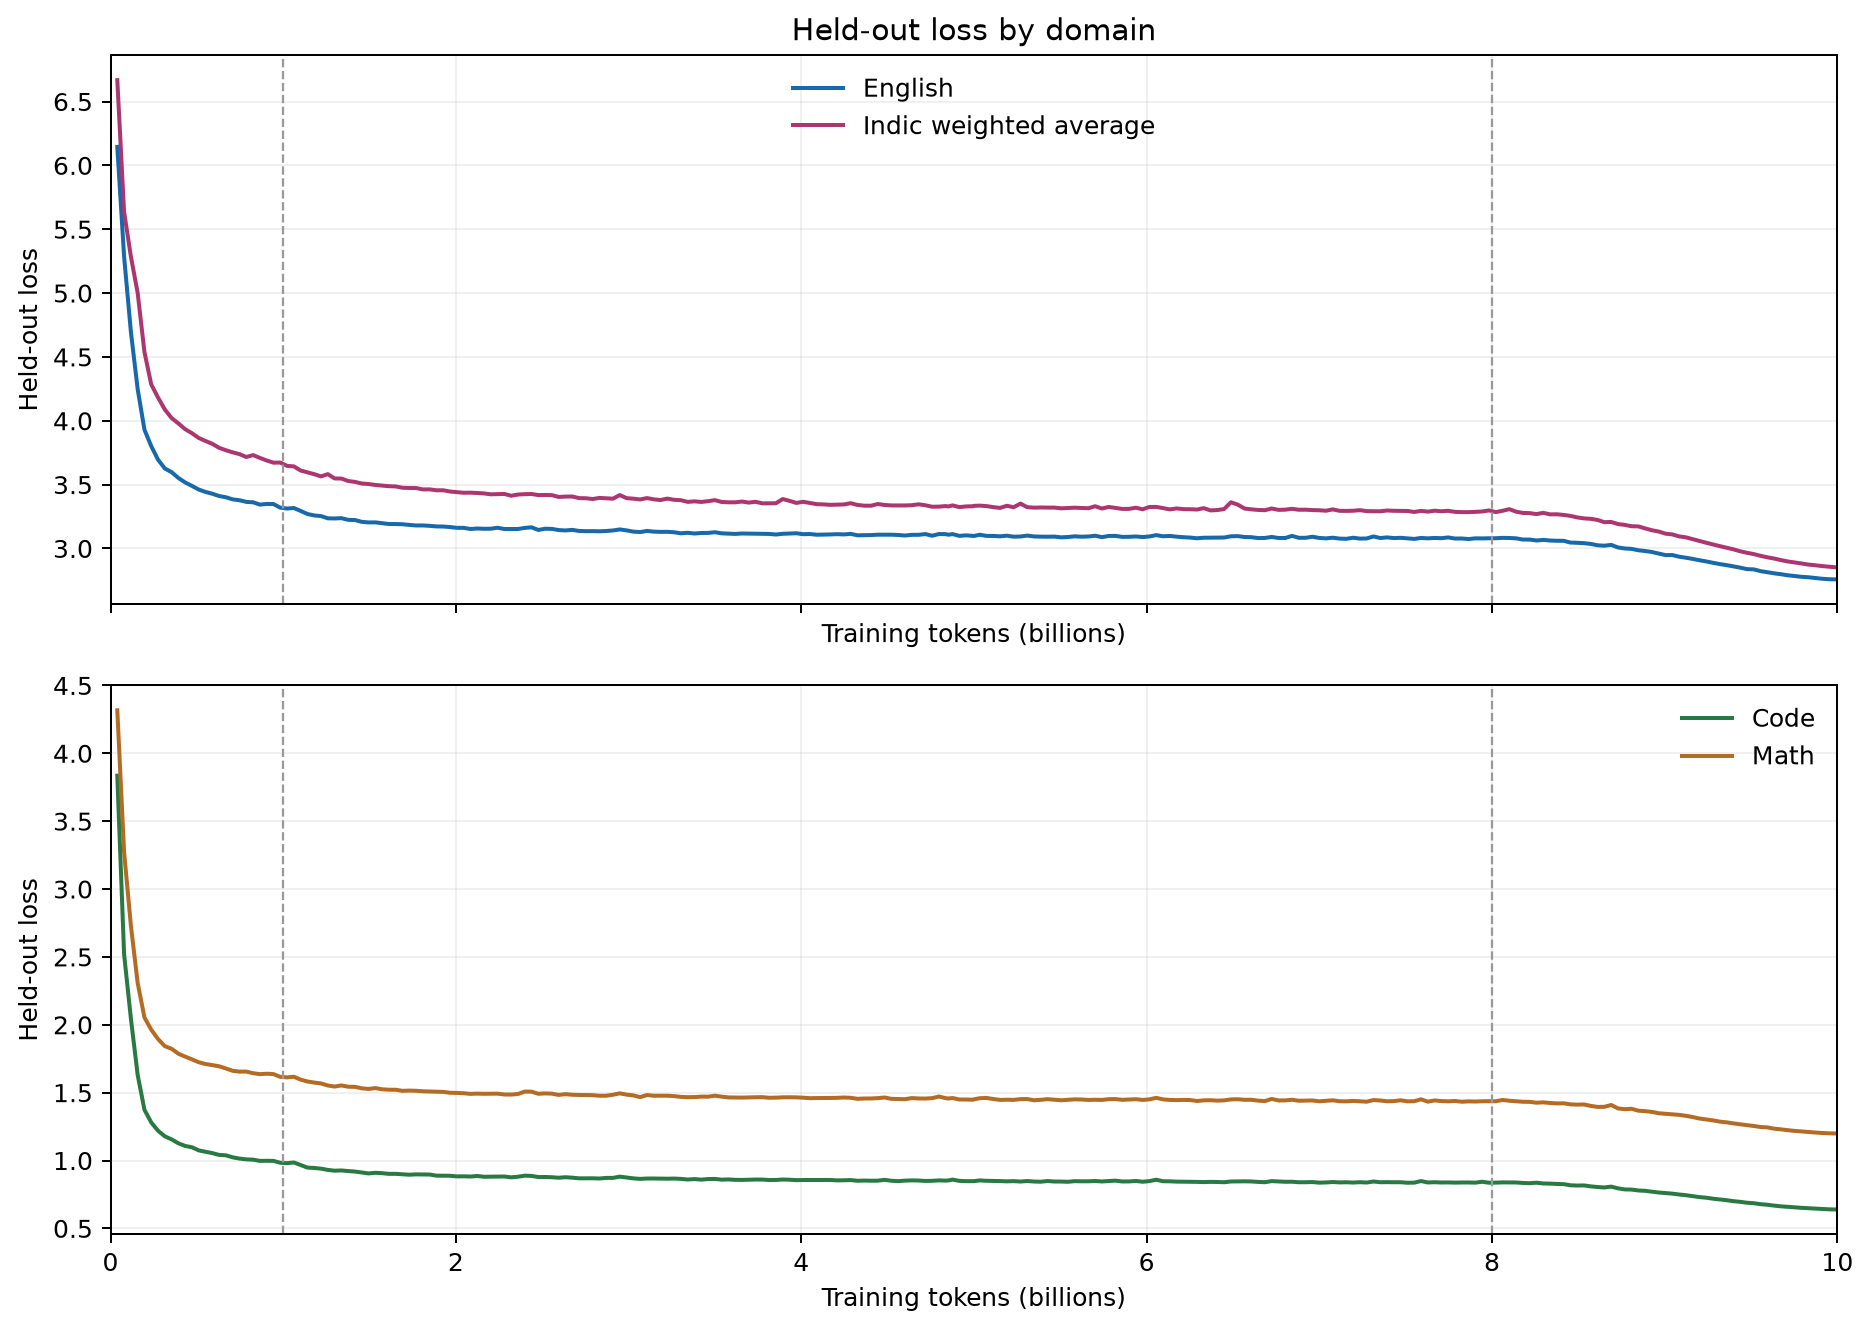
\includegraphics[width=0.96\linewidth]{figures/loss_domains.png}
\caption{Held-out losses for English, Indic, code, and math across training.}
\end{figure}

\begin{figure}[htbp]
\centering
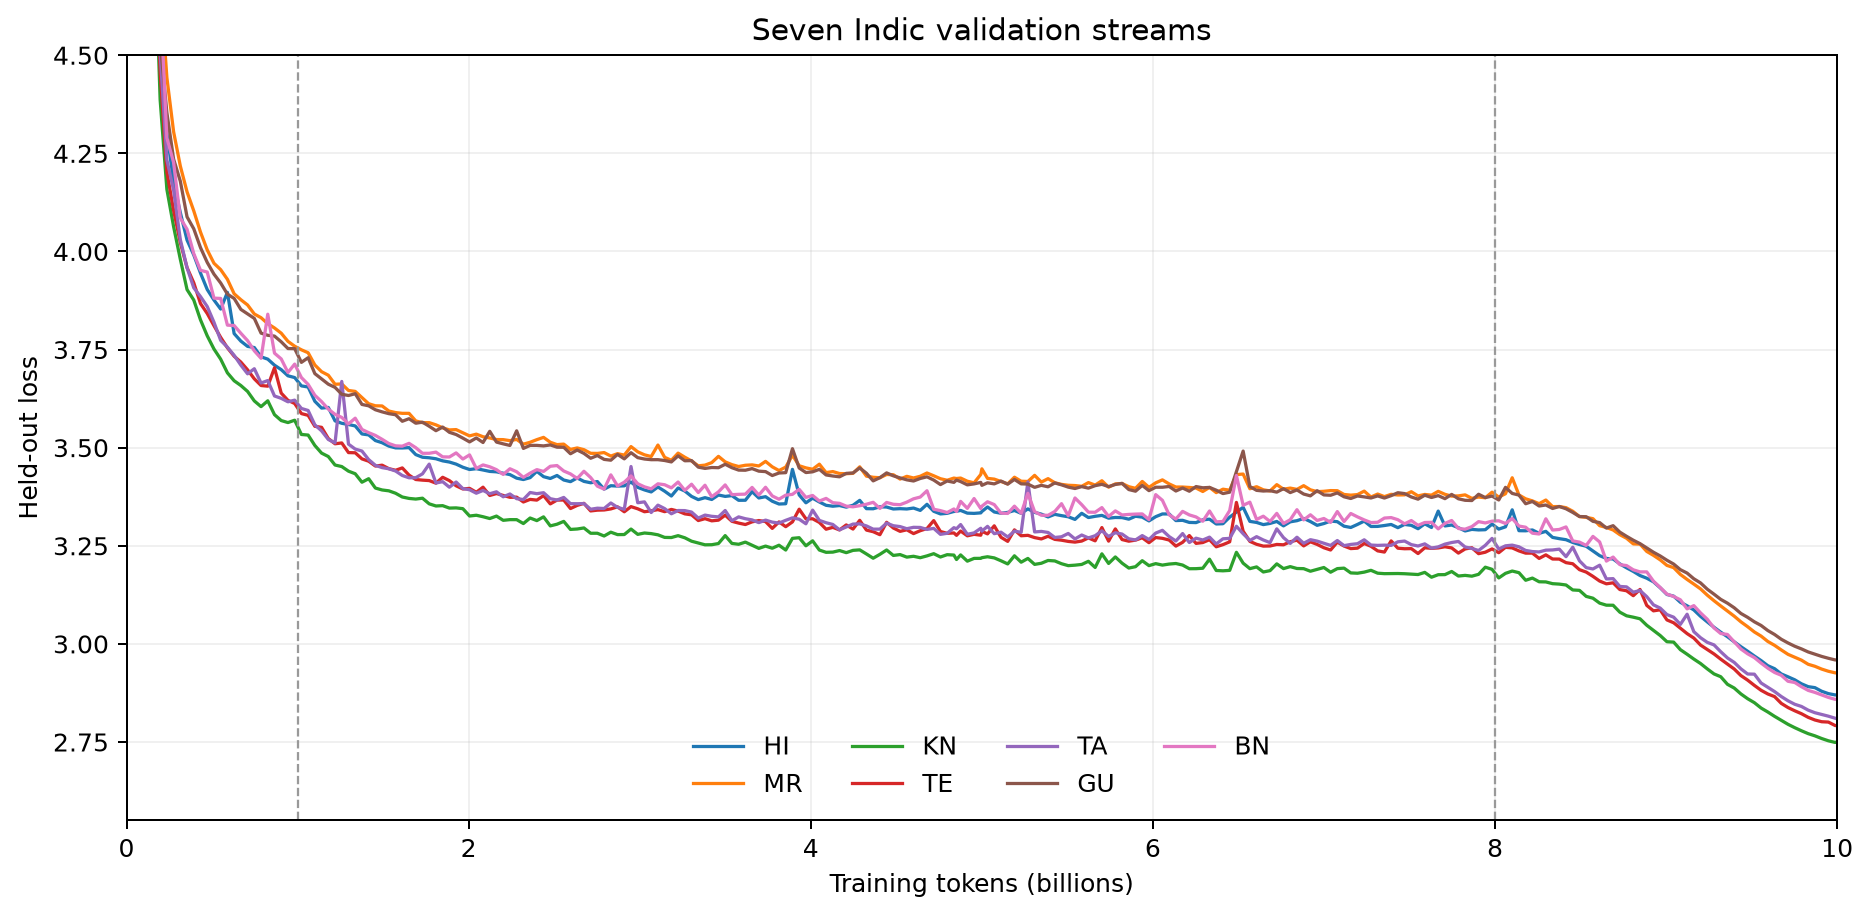
\includegraphics[width=0.96\linewidth]{figures/loss_indic.png}
\caption{Held-out loss trajectories for the seven Indic languages.}
\end{figure}

The final per-source validation losses are:

{
\begin{longtable}[]{@{}lrlr@{}}
\toprule\noalign{}
Source & Loss & Source & Loss \\
\midrule\noalign{}
\endhead
\bottomrule\noalign{}
\endlastfoot
English & 2.7597 & Code & 0.6389 \\
Math & 1.1989 & Hindi & 2.8699 \\
Marathi & 2.9260 & Kannada & 2.7501 \\
Telugu & 2.7916 & Tamil & 2.8090 \\
Gujarati & 2.9592 & Bengali & 2.8593 \\
\end{longtable}
}

\clearpage\section{Fixed prompt test on the final
checkpoint}\label{fixed-prompt-test-on-the-final-checkpoint}

I used the frozen tokenizer (SHA-256
\path{c53e0e95cd19e2954a8c7114c0a580eeb16698b153fdf84c5d80a7187d778d29})
and placed \texttt{\textless{}eod\textgreater{}} before each prompt to
begin a packed-style document. Decoding was \textbf{greedy
(\texttt{temperature=0})}, capped at 48 new tokens, with
\texttt{\textless{}eod\textgreater{}} as the stop token. None of the 23
completions emitted \texttt{\textless{}eod\textgreater{}} before the
cap. The checkpoint was SHA-verified before loading. The appendix
preserves the decoded text, with otherwise invisible trailing ASCII
spaces shown as \texttt{{[}space{]}}.

This probe ran on a \textbf{CPU reference}: each dense projection was
quantized once to the run\textquotesingle s blockwise FP8 E4M3 weight
representation, activations used the reference FP8 quantizer, and the
model used BF16 autocast with PyTorch SDPA attention. It preserves the
saved weights, tokenizer, architecture, and major quantization choices,
but does \textbf{not} execute H100 DeepGEMM, Triton fusion, or FA3. It
is a qualitative check, not an official downstream score or a bit-exact
native-GPU inference result. The repository\textquotesingle s
model/tokenizer files have not changed since the training commit.

Selected observations from the exact outputs in the appendix:

\begin{itemize}
\tightlist
\item
  Prompt format changes the result:
  \texttt{The\ capital\ of\ France\ is} continued incorrectly, while
  \texttt{Q:\ What\ is\ the\ capital\ of\ France?\textbackslash{}nA:}
  answered \textbf{Paris} and then repeated the Q\&A pair.
\item
  \texttt{2\ +\ 2\ =} began with \textbf{4}, but \texttt{12\ +\ 19\ =}
  began with \textbf{19} and the worked-example prompt answered
  \textbf{20}, both wrong.
\item
  \texttt{Water\ freezes\ at} produced \textbf{−18°C}. The Earth-orbit
  prompt started with \textbf{Sun}, then incorrectly claimed the Sun
  revolves around Earth.
\item
  A factorial prompt began with the correct recursive line, but
  continued into invalid top-level Python. The \texttt{add} and
  \texttt{is\_even} prompts produced docstring prose without a working
  function body within 48 tokens.
\item
  Text was generated in all seven Indic languages, but capital questions
  were inconsistent and several outputs looped. Tamil began with Delhi,
  followed by repeated punctuation; Hindi named Mumbai as
  India\textquotesingle s capital. Kannada and Gujarati produced text
  about Delhi without directly answering the cloze.
\end{itemize}

These are fixed, hand-selected examples, \textbf{not a statistically
representative benchmark}. They demonstrate a gap between next-token
prediction and reliable answers or executable code. Greedy decoding can
exaggerate loops; a tuned sampler may improve prose but cannot make an
incorrect factual answer correct by itself.

\section{Numerical and stability
audit}\label{numerical-and-stability-audit}

The final audit confirmed 25,432 contiguous per-update training records,
257 validation events, 2,546 sampled stability-probe updates, and
matching midpoint/final checkpoint receipts. It recorded \textbf{zero
non-finite incidents}, \textbf{zero training-loss spikes above twice the
preceding 20-update median}, and no non-finite values in any sampled
probe. Direct inspection found no non-finite model tensor in the final
checkpoint. The launch GPU suite passed 29 tests and the native
preflight passed; those checks establish execution/numerical readiness,
not downstream quality.

Gradient clipping occurred on 254 of 25,432 updates (1.0\%): 238 during
warmup, 16 during the stable phase, and \textbf{none during decay}. The
19 updates with a clipping coefficient below 0.1 were updates 1--19.
Pre-clip gradient norm had median 0.113, 99th percentile 0.995, and
maximum 16.05 early in training. This does not show a continuing
gradient explosion.

Across every sampled FP8 projection input, relative reconstruction RMS
error had median \textbf{2.43\%}, 99th percentile \textbf{2.65\%}, and
maximum \textbf{2.97\%}. No probe crossed the audit\textquotesingle s
10\% FP8-error cue; the maximum observed zero-code fraction was 0.45\%.
This is a sampled input-quantization measure, not a direct end-to-end
native-versus-BF16 quality comparison.

The audit counted 3,169 investigation alerts: 2,185 sampled attention
entropy values below 0.1, 270 sampled attention logits above 30, and 714
update-to-weight RMS ratios above 0.1. The high-logit alerts were
concentrated in warmup (260 of 270) and absent during decay. The
low-entropy cue persists, but its probe uses \textbf{the last query,
five heads, and only the last 128 keys}; a single sharply focused head
or that sampling rule can trigger it. It does not establish full-window
attention collapse.

All 714 update-ratio alerts came from
\texttt{layers.0.attn\_norm.weight}. Its saved full-vector RMS is
\textbf{0.01646}, versus 1.0 at initialization, and 46.7\% of its final
entries are negative. A small denominator makes an otherwise modest
update look large: near 5B tokens its sampled weight RMS was 0.0170,
update RMS 0.00178, and ratio 0.105. At the final update that ratio fell
to 0.0132. Other layer norms remained larger; for example, the final
layer\textquotesingle s attention-norm gain RMS is about 0.445. The
sampled layer-24 residual RMS rose from 0.61 initially to a maximum of
191, then fell to \textbf{34.37} by the end of decay. These values are
finite and the loss improved, but the scale migration should be tested
before assuming ternary QAT will behave normally from this checkpoint.

\begin{figure}[htbp]
\centering
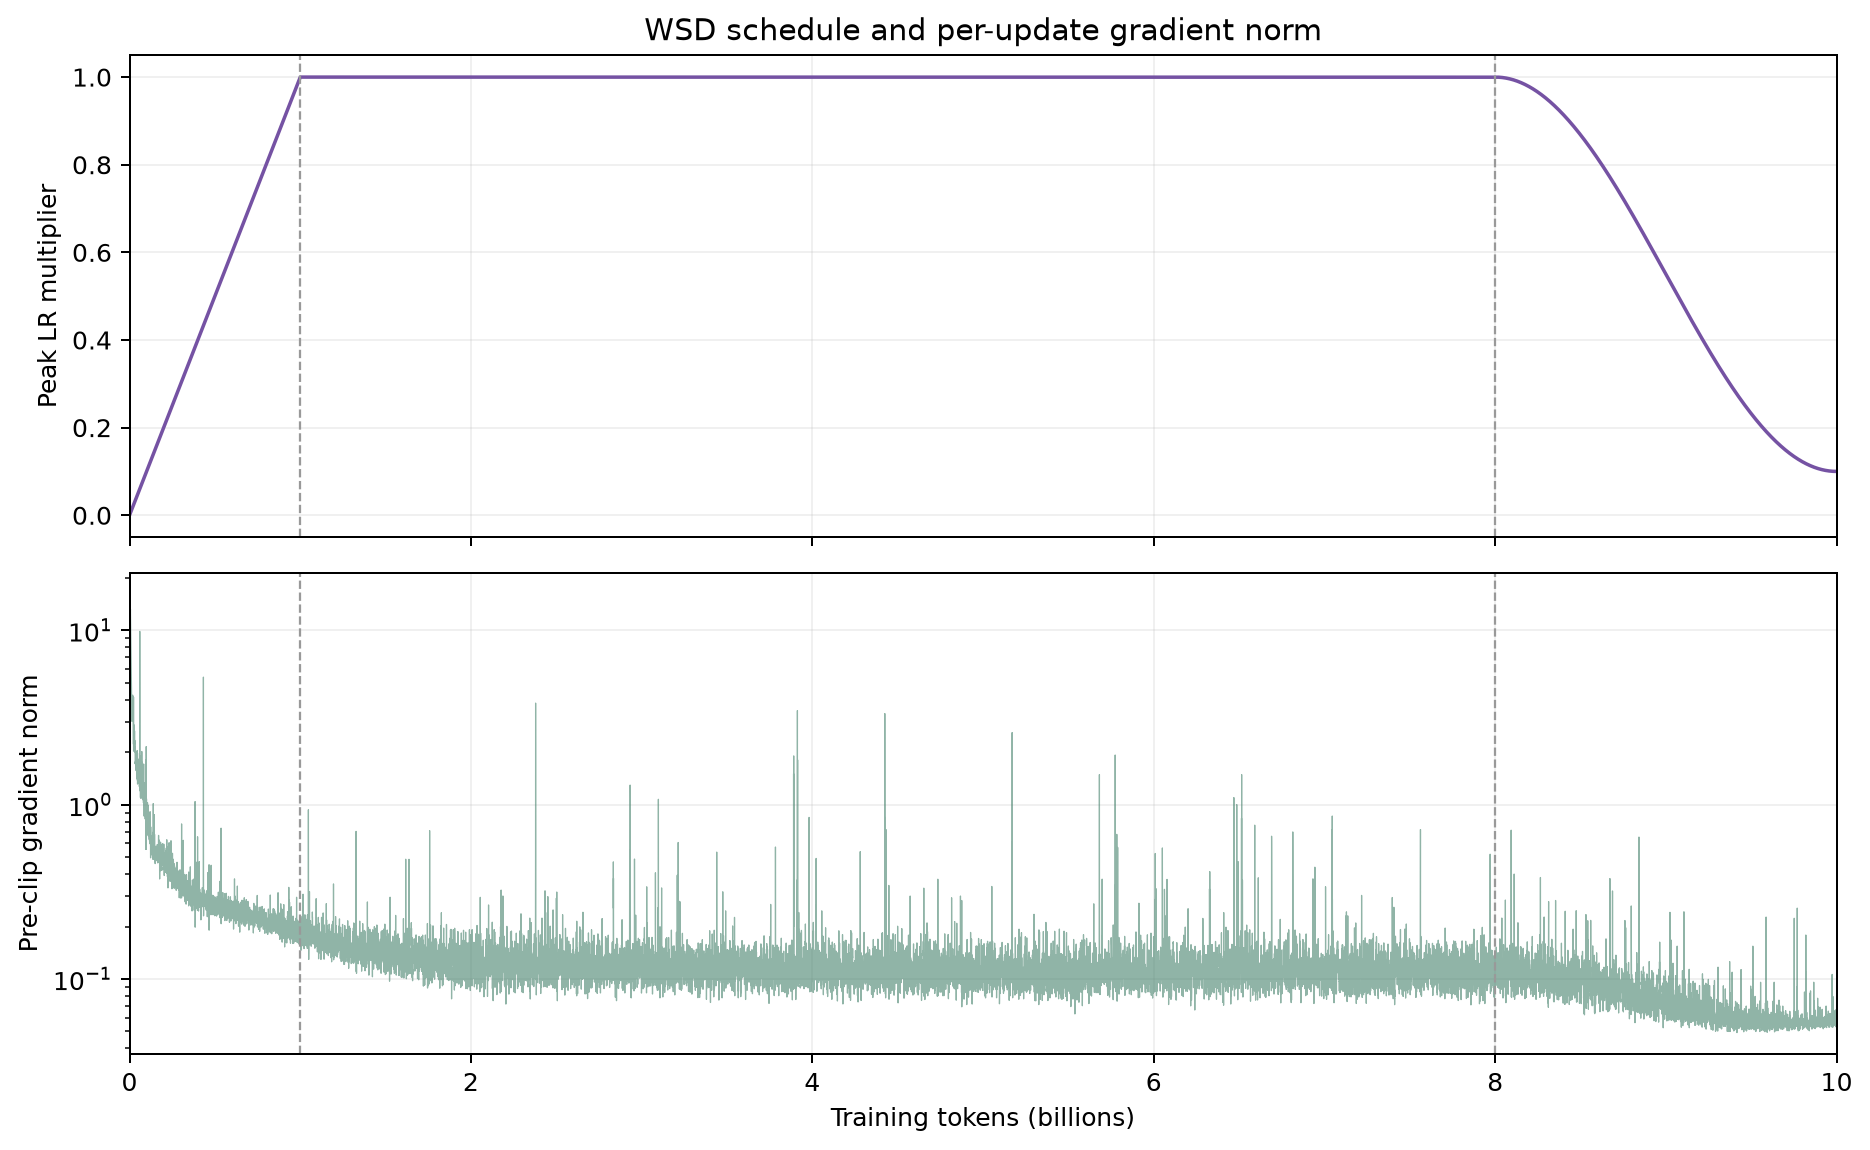
\includegraphics[width=0.96\linewidth]{figures/lr_gradient.png}
\caption{Learning-rate schedule, gradient norms, and clipping events.}
\end{figure}

\begin{figure}[htbp]
\centering
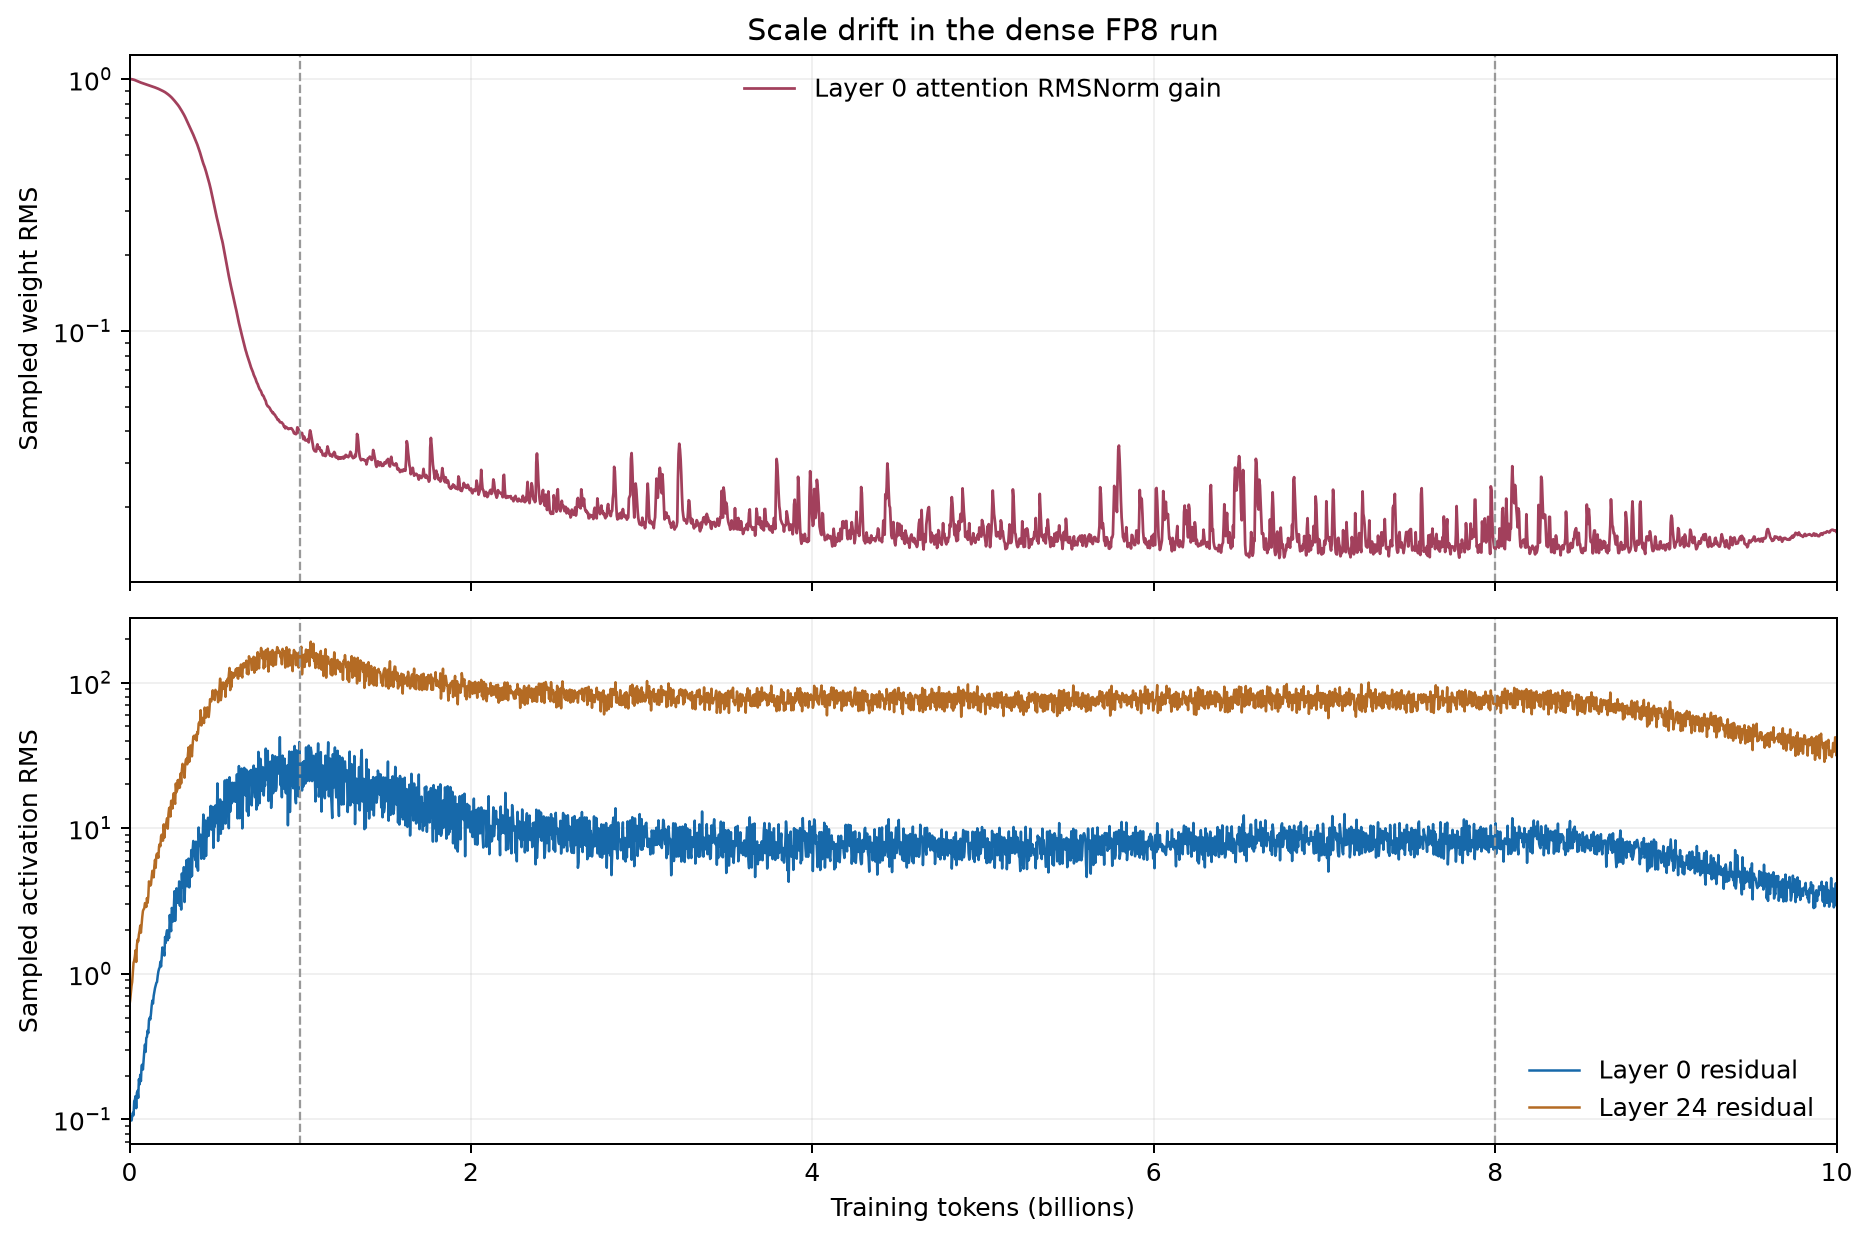
\includegraphics[width=0.96\linewidth]{figures/norm_residual_scales.png}
\caption{RMSNorm gain and sampled residual scales across training.}
\end{figure}

\begin{figure}[htbp]
\centering
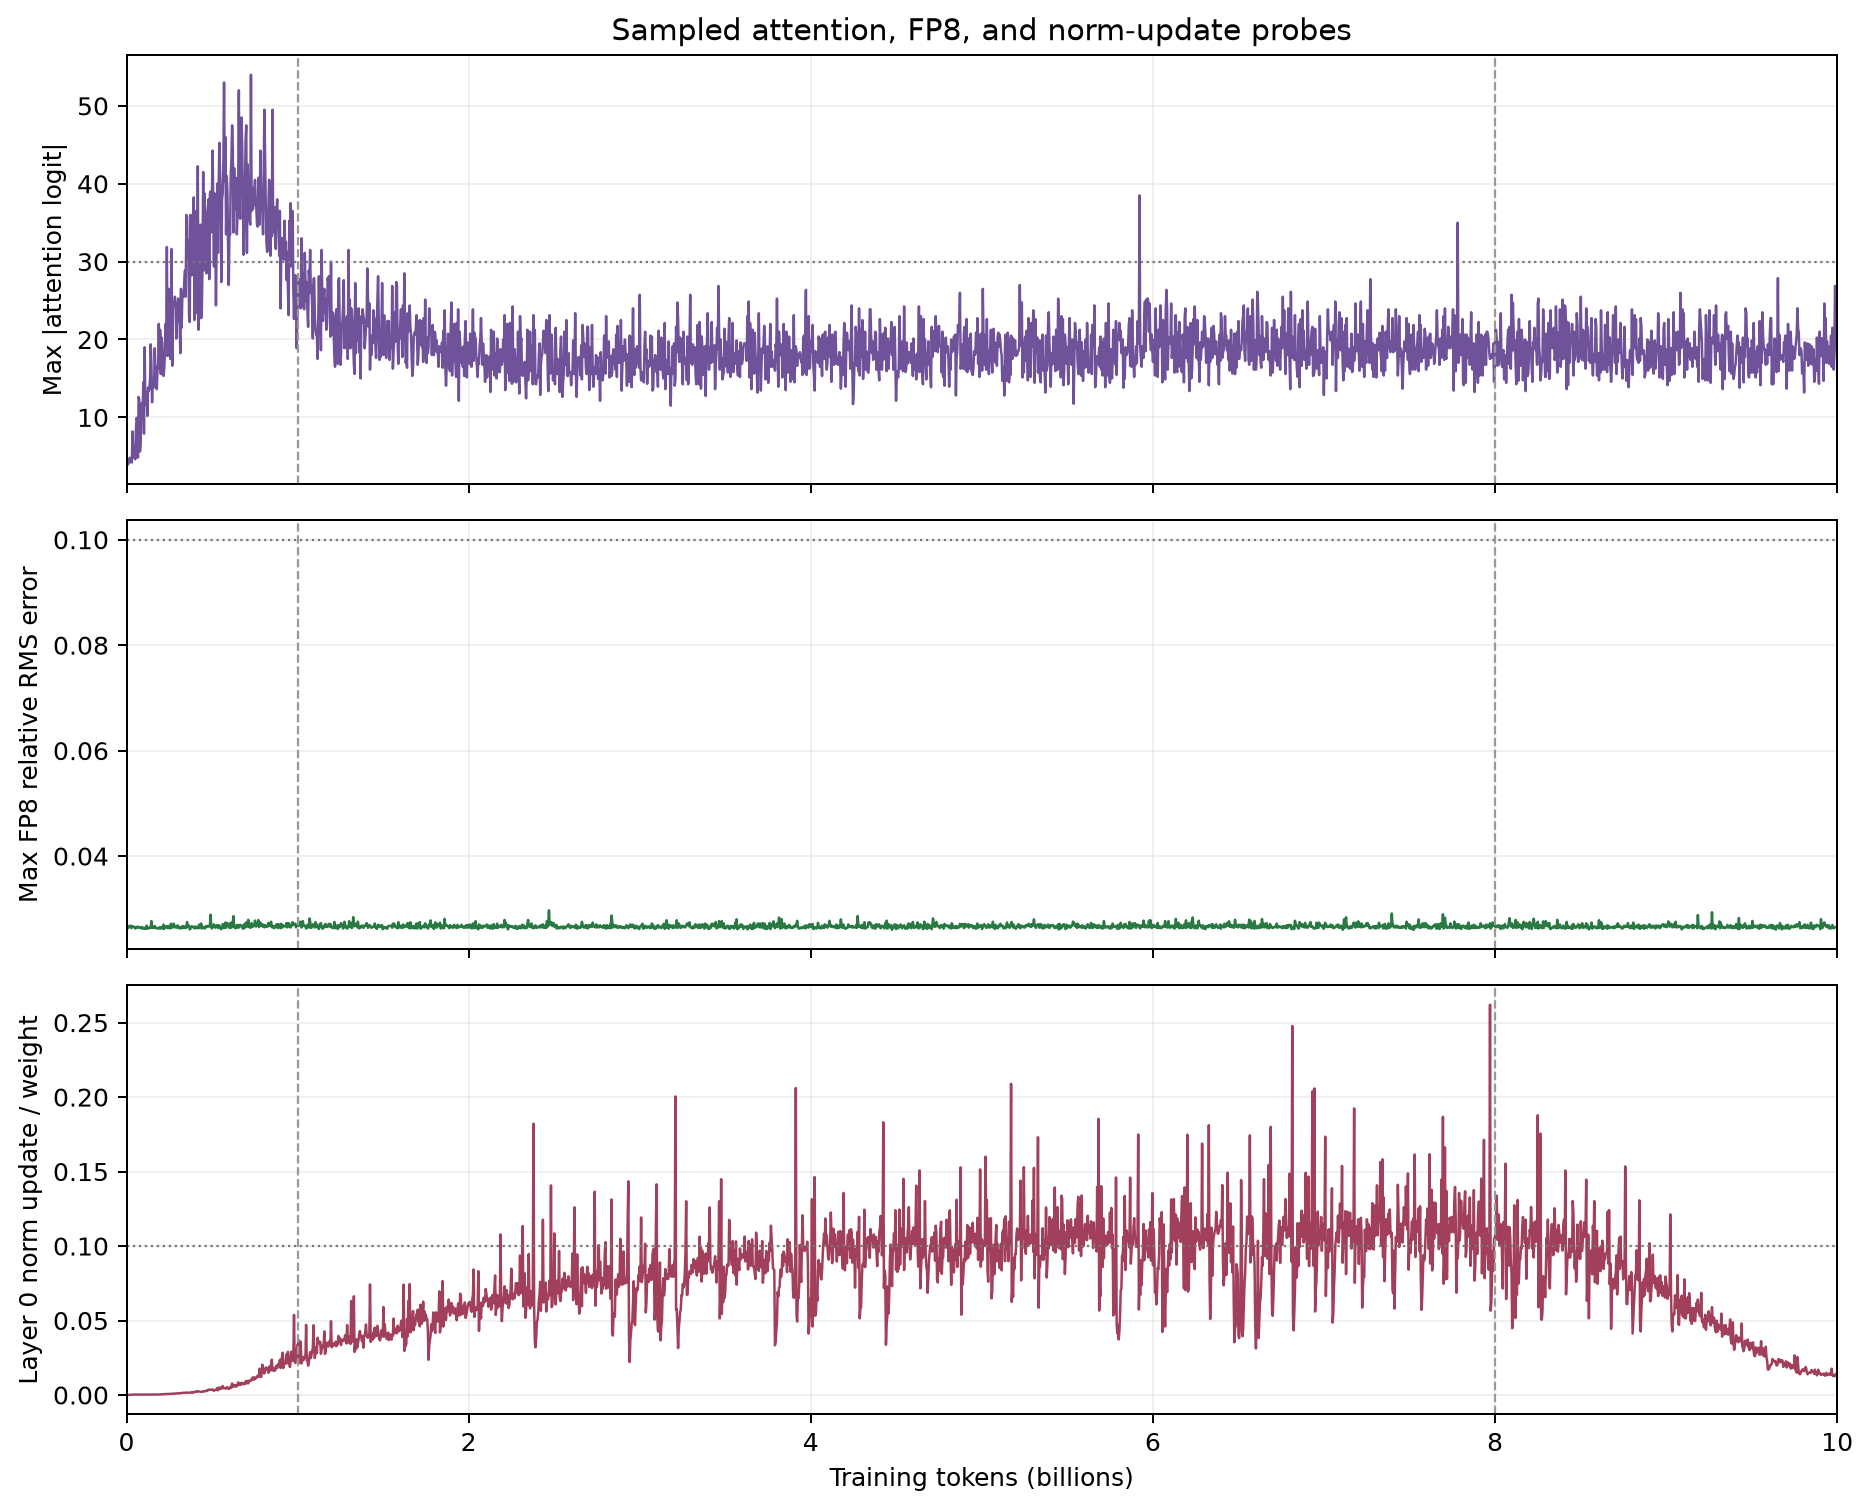
\includegraphics[width=0.96\linewidth]{figures/stability_signals.png}
\caption{Sampled attention, FP8 quantization, and update-to-weight diagnostics.}
\end{figure}

\begin{figure}[htbp]
\centering
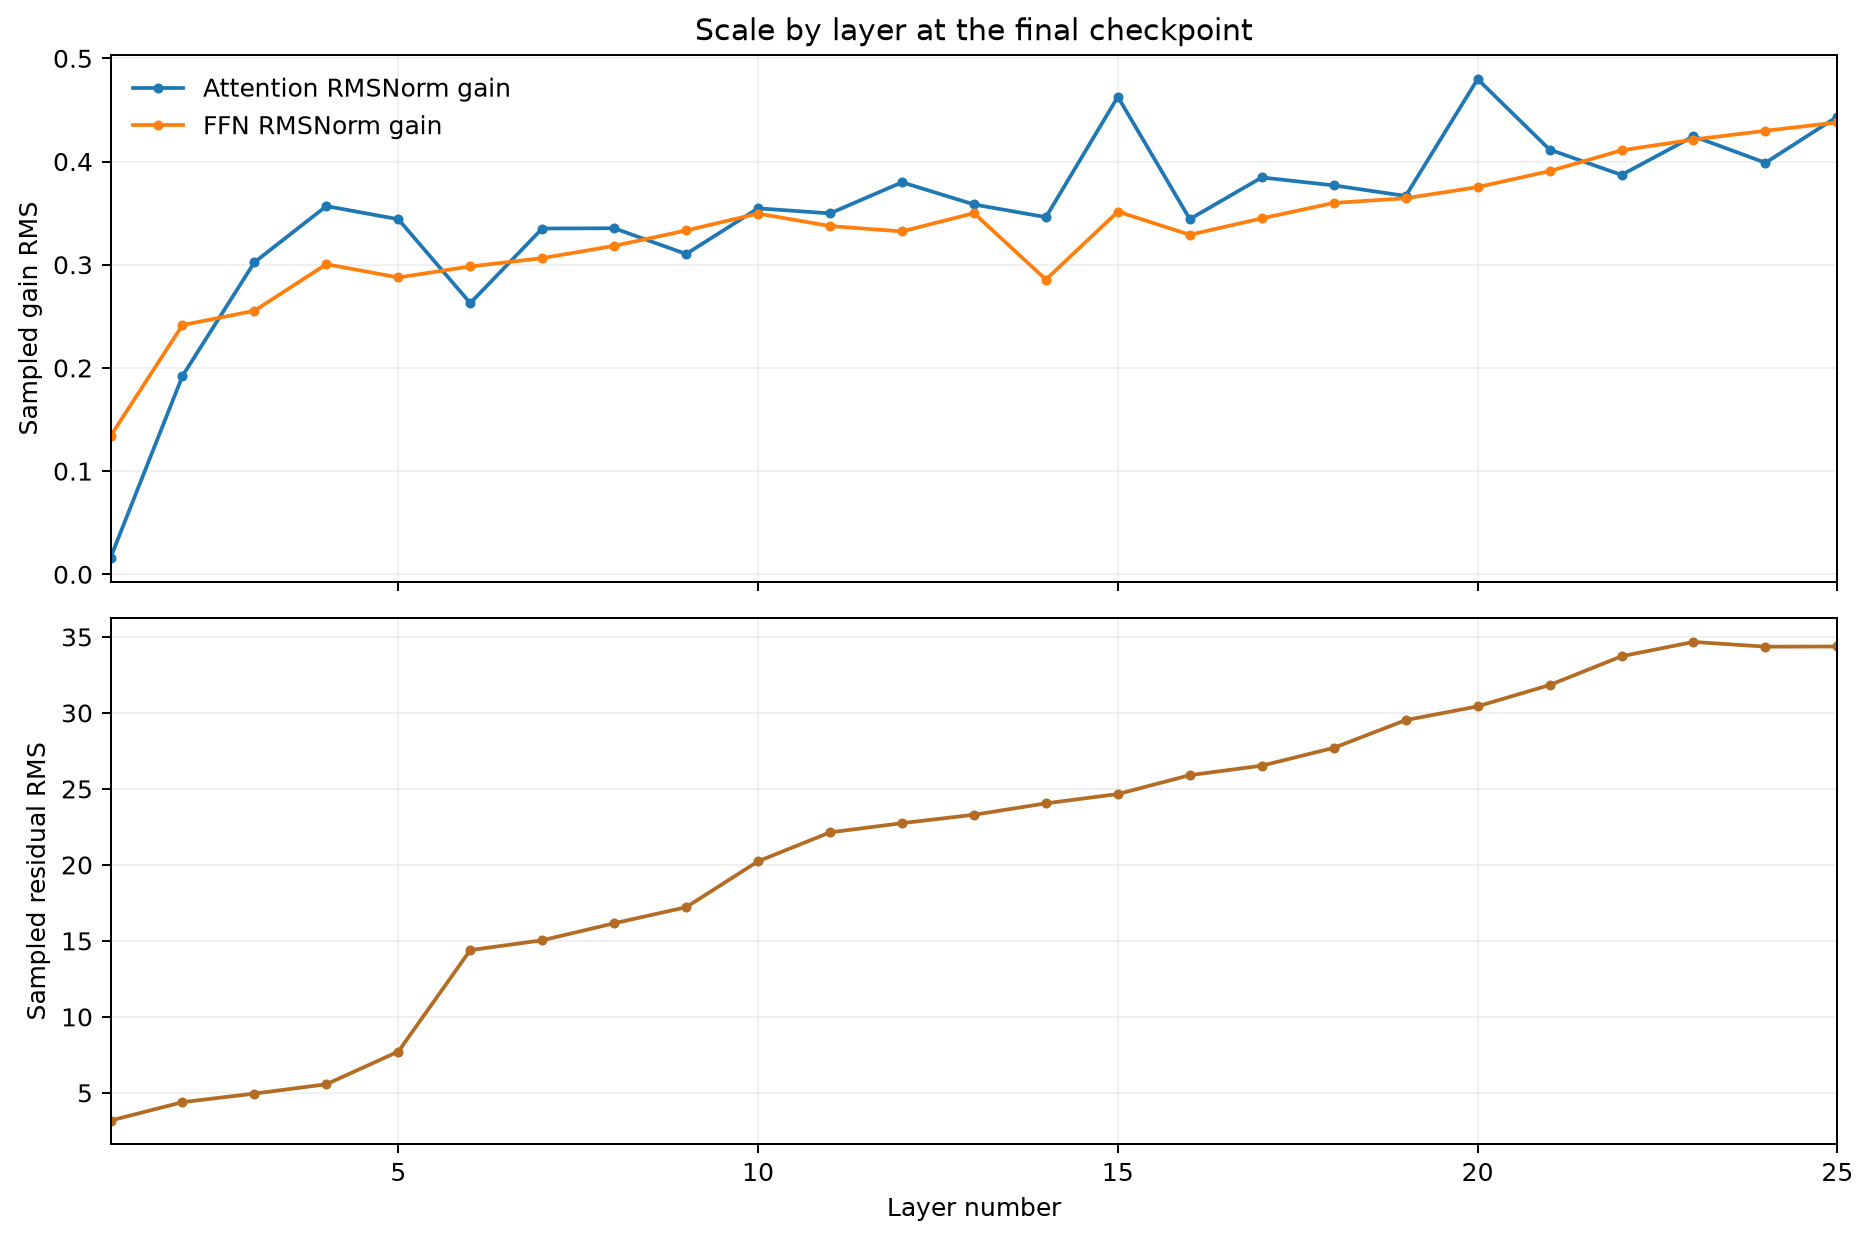
\includegraphics[width=0.96\linewidth]{figures/final_layer_scales.png}
\caption{Scale diagnostics by layer at the final checkpoint.}
\end{figure}

\clearpage\section{Time, throughput, and recording
integrity}\label{time-throughput-and-recording-integrity}

Training ran from \textbf{October 1, 7:06 p.m. IST} to \textbf{October
2, 4:23 p.m. IST}, in three recorded invocations. The first was
interrupted at update 12,339 / 4.852B tokens by the Azure shutdown
schedule; the VM remained deallocated for about \textbf{8 hours 10
minutes} before the exact-resume checkpoint was used. The planned
midpoint stop at update 12,716 / 5.000B tokens added about 38 seconds
between invocations. The final training and verification receipts are
complete, and the VM deallocated only after Blob size/MD5 verification.

The sum of the three \textbf{training-invocation wall times} is 13.11
hours, yielding \textbf{211,873 training tokens/s} including validation,
checkpointing, and training-process overhead. Median logged per-update
throughput after the initial 100 updates was \textbf{236,566 tokens/s}.
The 10.4\% difference is consistent with periodic evaluation, checkpoint
I/O, and other pauses; it is not a measured kernel-only overhead
attribution. Peak reported CUDA allocated memory was \textbf{84.37 GiB}
and peak reserved memory \textbf{87.71 GiB}. These invocation times are
not the entire Azure billing interval, which also includes VM
preparation and finalization.

Validation was frequent: 257 events × 15,728,640 scored tokens per event
= \textbf{4.04B held-out forward-pass tokens}. Those are not training
tokens and do not imply the same FLOP cost as backpropagation. The
recorded 100-update cadence was useful for diagnosing this pilot, but
future cost-sensitive searches can test a lower cadence while preserving
milestone and final evaluations.

\section{What this run does and does not
establish}\label{what-this-run-does-and-does-not-establish}

\begin{enumerate}
\def\labelenumi{\arabic{enumi}.}
\tightlist
\item
  \textbf{Established:} the dense FP8 stack completed 10B tokens with a
  resumable, audited checkpoint; held-out loss improved in all ten
  sources; the final checkpoint is archived and the VM is deallocated.
\item
  \textbf{Strong signal:} finishing the 2B-token decay mattered greatly
  for this trial. A controlled shorter/longer decay or lower peak-LR
  comparison is still needed to choose a recipe.
\item
  \textbf{Concern to test:} first-layer norm-gain collapse, large
  residual scales, and persistent focused-attention cues occurred
  despite finite gradients and falling loss. A small paired continuation
  or rerun with lower \textbf{auxiliary norm LR}, keeping data and
  projection LR fixed, would test the most direct hypothesis. Compare
  held-out loss, gain/residual trajectories, and the same prompt set; do
  not infer causality from this single run.
\item
  \textbf{Not established:} broad downstream ability, production
  inference quality, task-aware ModelTunnelv2 transfer, or QAT
  conversion quality. The prompt suite is illustrative and the CPU
  reference is not native H100 inference. Formal held-out task
  evaluation and a QAT branch should use the verified final checkpoint
  and preserve their own receipts.
\end{enumerate}

\section{Reproduction and source
files}\label{reproduction-and-source-files}

The raw verified run lives under Azure Blob
\texttt{runs/terminus\_lean\_150m\_10b\_run\_20261001/}. The final
checkpoint is also in the S3 run mirror. Raw logs, checkpoint tensors,
and corpora are intentionally \textbf{not committed} in this repository.
To reproduce the figures after downloading the named Blob files into one
run-root directory:

\begin{verbatim}
python -m pip install matplotlib numpy torch
python experiments/terminus_lean_150m_10b/analysis/analyze_final_run.py \
  --run-root /path/to/downloaded/run \
  --output-dir experiments/terminus_lean_150m_10b/analysis/figures
python experiments/terminus_lean_150m_10b/analysis/probe_final_checkpoint.py \
  --run-root /path/to/downloaded/run \
  --tokenizer tokenizer/tokenizer-65k.json \
  --output /path/to/prompt_results.json
\end{verbatim}

The analysis consumed \path{dense/events.jsonl},
\path{dense/stability.jsonl}, \texttt{audit\_final.json},
\path{views/manifest.dense.json}, \texttt{config.json},
\texttt{dense/run.json}, the final checkpoint/receipt, the frozen
tokenizer, and launch/finalizer receipts. Numeric summaries used to draw
the figures are in \url{figures/metrics.json}. Validation source
exposure is specified by the manifest, while the event log does not
record each training document\textquotesingle s realized source
identity. The stability probe samples the first microbatch on selected
updates and cannot rule out unobserved brief events between samples.

\clearpage
\appendix\section{All fixed prompt completions}
Each completion is the decoded 48-token greedy output from the SHA-verified final checkpoint. The visible marker \texttt{[space]} represents a trailing ASCII space; prompts and completions are separate. These fixed examples are qualitative probes, not a task benchmark.
\filbreak
\subsection*{1. France capital cloze (english\_fact)}
\addcontentsline{toc}{subsection}{1. France capital cloze (english\_fact)}
\textbf{Prompt}\par
\begin{quote}\small\raggedright  The capital of France is\par\end{quote}
\textbf{Completion} (48 new tokens)\par
\begin{quote}\small\raggedright  \hspace*{0.5em}the capital of the United States. The United States is the largest country in the world. The United States is the largest country in the world. The United States is the largest country in the world. The United States is the largest country in\par\end{quote}
\filbreak
\subsection*{2. India capital cloze (english\_fact)}
\addcontentsline{toc}{subsection}{2. India capital cloze (english\_fact)}
\textbf{Prompt}\par
\begin{quote}\small\raggedright  The capital of India is\par\end{quote}
\textbf{Completion} (48 new tokens)\par
\begin{quote}\small\raggedright  \hspace*{0.5em}known for its rich cultural heritage and stunning natural beauty. However, the country faces challenges in its quest for sustainable development. One of the most pressing concerns is the issue of land degradation. Land degradation is a major issue in India, and it\par\end{quote}
\filbreak
\subsection*{3. Earth orbit cloze (english\_fact)}
\addcontentsline{toc}{subsection}{3. Earth orbit cloze (english\_fact)}
\textbf{Prompt}\par
\begin{quote}\small\raggedright  The Earth revolves around the\par\end{quote}
\textbf{Completion} (48 new tokens)\par
\begin{quote}\small\raggedright  \hspace*{0.5em}Sun, and the Sun revolves around the Earth. The Earth revolves around the Sun, and the Earth revolves around the Sun. The Earth revolves around the Sun, and the Earth revolves around the Sun. The Earth rev\par\end{quote}
\filbreak
\subsection*{4. Freezing point cloze (english\_fact)}
\addcontentsline{toc}{subsection}{4. Freezing point cloze (english\_fact)}
\textbf{Prompt}\par
\begin{quote}\small\raggedright  Water freezes at\par\end{quote}
\textbf{Completion} (48 new tokens)\par
\begin{quote}\small\raggedright  \hspace*{0.5em}-18°C, so the temperature of the water is -18°C. The temperature of the water is -18°C.\par\noindent \mbox{}\par\noindent The temperature of the water is -18°C\par\end{quote}
\filbreak
\subsection*{5. France capital QA (english\_qa)}
\addcontentsline{toc}{subsection}{5. France capital QA (english\_qa)}
\textbf{Prompt}\par
\begin{quote}\small\raggedright  Q: What is the capital of France?\par\noindent A:\par\end{quote}
\textbf{Completion} (48 new tokens)\par
\begin{quote}\small\raggedright  \hspace*{0.5em}The capital of France is Paris.\par\noindent Q: What is the capital of France?\par\noindent A: The capital of France is Paris.\par\noindent Q: What is the capital of France?\par\noindent A: The capital of France is Paris.\par\noindent \mbox{}\par\end{quote}
\filbreak
\subsection*{6. Week days QA (english\_qa)}
\addcontentsline{toc}{subsection}{6. Week days QA (english\_qa)}
\textbf{Prompt}\par
\begin{quote}\small\raggedright  Q: How many days are there in a week?\par\noindent A:\par\end{quote}
\textbf{Completion} (48 new tokens)\par
\begin{quote}\small\raggedright  \hspace*{0.5em}There are 24 hours in a week.\par\noindent Q: What is the difference between a day and a week?\par\noindent A: A day is a time, while a week is a time.\par\noindent Q: What is the difference between\par\end{quote}
\filbreak
\subsection*{7. Two plus two (math)}
\addcontentsline{toc}{subsection}{7. Two plus two (math)}
\textbf{Prompt}\par
\begin{quote}\small\raggedright  2 + 2 =\par\end{quote}
\textbf{Completion} (48 new tokens)\par
\begin{quote}\small\raggedright  \hspace*{0.5em}4\par\noindent \mbox{}\par\noindent 2 + 2 = 4\par\noindent \mbox{}\par\noindent 2 + 2 = 4\par\noindent \mbox{}\par\noindent 2 + 2 = 4\par\noindent \mbox{}\par\noindent 2 + 2 = 4\par\noindent \mbox{}\par\noindent \mbox{}\par\end{quote}
\filbreak
\subsection*{8. Twelve plus nineteen (math)}
\addcontentsline{toc}{subsection}{8. Twelve plus nineteen (math)}
\textbf{Prompt}\par
\begin{quote}\small\raggedright  12 + 19 =\par\end{quote}
\textbf{Completion} (48 new tokens)\par
\begin{quote}\small\raggedright  \hspace*{0.5em}19\par\noindent \mbox{}\par\noindent 12 + 19 = 19\par\noindent \mbox{}\par\noindent 12 + 19 = 19\par\noindent \mbox{}\par\noindent 12 + 19 = 19\par\noindent \mbox{}\par\noindent 1\par\end{quote}
\filbreak
\subsection*{9. Square root (math)}
\addcontentsline{toc}{subsection}{9. Square root (math)}
\textbf{Prompt}\par
\begin{quote}\small\raggedright  The square root of 81 is\par\end{quote}
\textbf{Completion} (48 new tokens)\par
\begin{quote}\small\raggedright  \hspace*{0.5em}approximately 1.4141.\par\noindent \mbox{}\par\noindent The square root of 81 is approximately 1.4141.\par\noindent \mbox{}\par\noindent The square root of 81 is approximately 1.4141.\par\noindent \mbox{}\par\end{quote}
\filbreak
\subsection*{10. Few-shot arithmetic (math)}
\addcontentsline{toc}{subsection}{10. Few-shot arithmetic (math)}
\textbf{Prompt}\par
\begin{quote}\small\raggedright  Question: What is 2 + 3?\par\noindent Answer: 5\par\noindent \mbox{}\par\noindent Question: What is 7 + 4?\par\noindent Answer: 11\par\noindent \mbox{}\par\noindent Question: What is 12 + 19?\par\noindent Answer:\par\end{quote}
\textbf{Completion} (48 new tokens)\par
\begin{quote}\small\raggedright  \hspace*{0.5em}20\par\noindent \mbox{}\par\noindent Question: What is 12 + 19?\par\noindent Answer: 20\par\noindent \mbox{}\par\noindent Question: What is 12 + 19?\par\noindent Answer: 20\par\noindent \mbox{}\par\noindent Question\par\end{quote}
\filbreak
\subsection*{11. Add function (code)}
\addcontentsline{toc}{subsection}{11. Add function (code)}
\textbf{Prompt}\par
\begin{quote}\small\raggedright \ttfamily def add(a, b):\par\noindent [space][space][space][space]\par\end{quote}
\textbf{Completion} (48 new tokens)\par
\begin{quote}\small\raggedright \ttfamily """\par\noindent \hspace*{2.0em}Add two integers a and b to a list in-place.\par\noindent \hspace*{2.0em}The function modifies the input list so that each element\par\noindent \hspace*{2.0em}is replaced by the sum of the two numbers.\par\noindent \hspace*{2.0em}The algorithm uses a stack to process the\par\end{quote}
\filbreak
\subsection*{12. Parity function (code)}
\addcontentsline{toc}{subsection}{12. Parity function (code)}
\textbf{Prompt}\par
\begin{quote}\small\raggedright \ttfamily def is\_even(n):\par\noindent [space][space][space][space]\par\end{quote}
\textbf{Completion} (48 new tokens)\par
\begin{quote}\small\raggedright \ttfamily """Return True if n is an even integer.\par\noindent \hspace*{2.0em}The function validates that `n` is a non‑negative integer;\par\noindent \hspace*{2.0em}if not, it raises a ValueError.\par\noindent \hspace*{2.0em}>>> is\_even(10): True\par\noindent [space][space][space][space]\par\end{quote}
\filbreak
\subsection*{13. Factorial continuation (code)}
\addcontentsline{toc}{subsection}{13. Factorial continuation (code)}
\textbf{Prompt}\par
\begin{quote}\small\raggedright \ttfamily def factorial(n):\par\noindent \hspace*{2.0em}if n <= 1:\par\noindent \hspace*{4.0em}return 1\par\noindent [space][space][space][space]\par\end{quote}
\textbf{Completion} (48 new tokens)\par
\begin{quote}\small\raggedright \ttfamily else:\par\noindent \hspace*{4.0em}return n * factorial(n - 1)\par\noindent \mbox{}\par\noindent \# Example usage:\par\noindent if n == 1:\par\noindent \hspace*{2.0em}return 1\par\noindent else:\par\noindent \hspace*{2.0em}return 1\par\noindent \mbox{}\par\noindent \# Return the factorial of[space]\par\end{quote}
\filbreak
\subsection*{14. Story continuation (english\_prose)}
\addcontentsline{toc}{subsection}{14. Story continuation (english\_prose)}
\textbf{Prompt}\par
\begin{quote}\small\raggedright  Once upon a time, a small fox entered a forest and\par\end{quote}
\textbf{Completion} (48 new tokens)\par
\begin{quote}\small\raggedright  \hspace*{0.5em}started to explore its surroundings. It was curious about what it was doing and how it could help humans.\par\noindent \mbox{}\par\noindent As it approached, the fox began to investigate its surroundings. It looked around and saw a small tree with branches and leaves.\par\end{quote}
\filbreak
\subsection*{15. Internet history (english\_prose)}
\addcontentsline{toc}{subsection}{15. Internet history (english\_prose)}
\textbf{Prompt}\par
\begin{quote}\small\raggedright  The history of the Internet began with\par\end{quote}
\textbf{Completion} (48 new tokens)\par
\begin{quote}\small\raggedright  \hspace*{0.5em}the invention of the Internet in 1909. The first Internet was created by the United States government. The first Internet was created by the United States government. The first Internet was created by the United States government. The first Internet\par\end{quote}
\filbreak
\subsection*{16. India capital Hindi (hindi)}
\addcontentsline{toc}{subsection}{16. India capital Hindi (hindi)}
\textbf{Prompt}\par
\begin{quote}\small\raggedright \devanagarifont भारत की राजधानी है\par\end{quote}
\textbf{Completion} (48 new tokens)\par
\begin{quote}\small\raggedright \devanagarifont मुंबई। मुंबई के अलावा देश के अन्य शहरों में भी लोग रहते हैं। मुंबई में कई तरह के होटल और रेस्टॉरेंट हैं। मुंबई में कई तरह के रेस्टॉरेंट हैं। मुंबई में कई तरह के रेस्टॉरेंट हैं। मुंबई\par\end{quote}
\filbreak
\subsection*{17. Maharashtra capital Hindi (hindi)}
\addcontentsline{toc}{subsection}{17. Maharashtra capital Hindi (hindi)}
\textbf{Prompt}\par
\begin{quote}\small\raggedright \devanagarifont भारत की राजधानी नई दिल्ली है। महाराष्ट्र की राजधानी\par\end{quote}
\textbf{Completion} (48 new tokens)\par
\begin{quote}\small\raggedright \devanagarifont है। महाराष्ट्र के मुख्यमंत्री एकनाथ शिंदे ने 2014 में महाराष्ट्र के मुख्यमंत्री के रूप में शपथ ली थी।\par\noindent \hspace*{0.5em}महाराष्ट्र के मुख्यमंत्री एकनाथ शिंदे ने 2014 में महाराष्ट्र के मुख्यमंत्री के रूप में शपथ ली थी।\par\noindent [space]\par\end{quote}
\filbreak
\subsection*{18. Maharashtra capital Marathi (marathi)}
\addcontentsline{toc}{subsection}{18. Maharashtra capital Marathi (marathi)}
\textbf{Prompt}\par
\begin{quote}\small\raggedright \devanagarifont महाराष्ट्राची राजधानी\par\end{quote}
\textbf{Completion} (48 new tokens)\par
\begin{quote}\small\raggedright \devanagarifont मुंबईत आज (19 जून) दुपारी 12. 30 वाजता राष्ट्रवादी काँग्रेसचे अध्यक्ष शरद पवार यांची मुंबईत जाहीर सभा होणार आहे. या सभेत राष्ट्रवादी काँग्रेसचे नेते आणि खासदार छगन\par\end{quote}
\filbreak
\subsection*{19. Bangladesh capital Bengali (bengali)}
\addcontentsline{toc}{subsection}{19. Bangladesh capital Bengali (bengali)}
\textbf{Prompt}\par
\begin{quote}\small\raggedright \bengalifont বাংলাদেশের রাজধানী\par\end{quote}
\textbf{Completion} (48 new tokens)\par
\begin{quote}\small\raggedright \bengalifont \hspace*{0.5em}ঢাকায় অবস্থিত বাংলাদেশ হাইকমিশন অব ইন্ডাস্ট্রিজ (বিএইচআইসি) এর উদ্যোগে 'বাংলাদেশের হাইকমিশন অব ইন্ডাস্ট্রিজ' (বি\par\end{quote}
\filbreak
\subsection*{20. India capital Kannada (kannada)}
\addcontentsline{toc}{subsection}{20. India capital Kannada (kannada)}
\textbf{Prompt}\par
\begin{quote}\small\raggedright \kannadafont ಭಾರತದ ರಾಜಧಾನಿ\par\end{quote}
\textbf{Completion} (48 new tokens)\par
\begin{quote}\small\raggedright \kannadafont \hspace*{0.5em}ದೆಹಲಿಯಲ್ಲಿ ದೆಹಲಿ ದೆಹಲಿ ಎಂಬ ಹೆಸರಿನಿಂದ ಕರೆಯಲ್ಪಡುವ ದೆಹಲಿ ದೆಹಲಿ ಎಂಬ ಹೆಸರಿನಿಂದ ಕರೆಯಲ್ಪಡುವ ದೆಹಲಿ ದೆಹಲಿ ಎಂಬ ಹೆಸರಿನಿಂದ ಕರೆಯಲ್ಪಡುವ ದೆಹಲಿ ದೆಹ\par\end{quote}
\filbreak
\subsection*{21. India capital Gujarati (gujarati)}
\addcontentsline{toc}{subsection}{21. India capital Gujarati (gujarati)}
\textbf{Prompt}\par
\begin{quote}\small\raggedright \gujaratifont ભારતની રાજધાની\par\end{quote}
\textbf{Completion} (48 new tokens)\par
\begin{quote}\small\raggedright \gujaratifont દિલ્હીમાં એક ચોંકાવનારો કિસ્સો સામે આવ્યો છે. અહીં એક વ્યક્તિએ પોતાના ઘરેથી 1000 રૂપિયા લીધા અને પછી તે પૈસા પરત નહી કરે. આ વ્યક્તિએ પોતાના ઘરેથી 10\par\end{quote}
\filbreak
\subsection*{22. India capital Tamil (tamil)}
\addcontentsline{toc}{subsection}{22. India capital Tamil (tamil)}
\textbf{Prompt}\par
\begin{quote}\small\raggedright \tamilfont இந்தியாவின் தலைநகரம்\par\end{quote}
\textbf{Completion} (48 new tokens)\par
\begin{quote}\small\raggedright \tamilfont டெல்லி. . . . . . . . . . . . . . . . . . . . . . . . . . . . . . . . . . . . . . . . . . . . . .\par\end{quote}
\filbreak
\subsection*{23. India capital Telugu (telugu)}
\addcontentsline{toc}{subsection}{23. India capital Telugu (telugu)}
\textbf{Prompt}\par
\begin{quote}\small\raggedright \telugufont భారతదేశ రాజధాని\par\end{quote}
\textbf{Completion} (48 new tokens)\par
\begin{quote}\small\raggedright \telugufont \hspace*{0.5em}ఢిల్లీలో ఢిల్లీ మెట్రోపాలిటన్ డెవలప్మెంట్ అథారిటీ (డీఎండీఏ) ఢిల్లీ మెట్రోపాలిటన్ డెవలప్మెంట్ అథారిటీ (డీఎండీఏ)[space]\par\end{quote}
\end{document}
